\documentclass{standalone}
\usepackage{tikz}
\usetikzlibrary{patterns, positioning}
\usepackage[sfdefault]{ClearSans} %% option 'sfdefault' activates Clear Sans as the default text font
\usepackage[T1]{fontenc}

\begin{document}
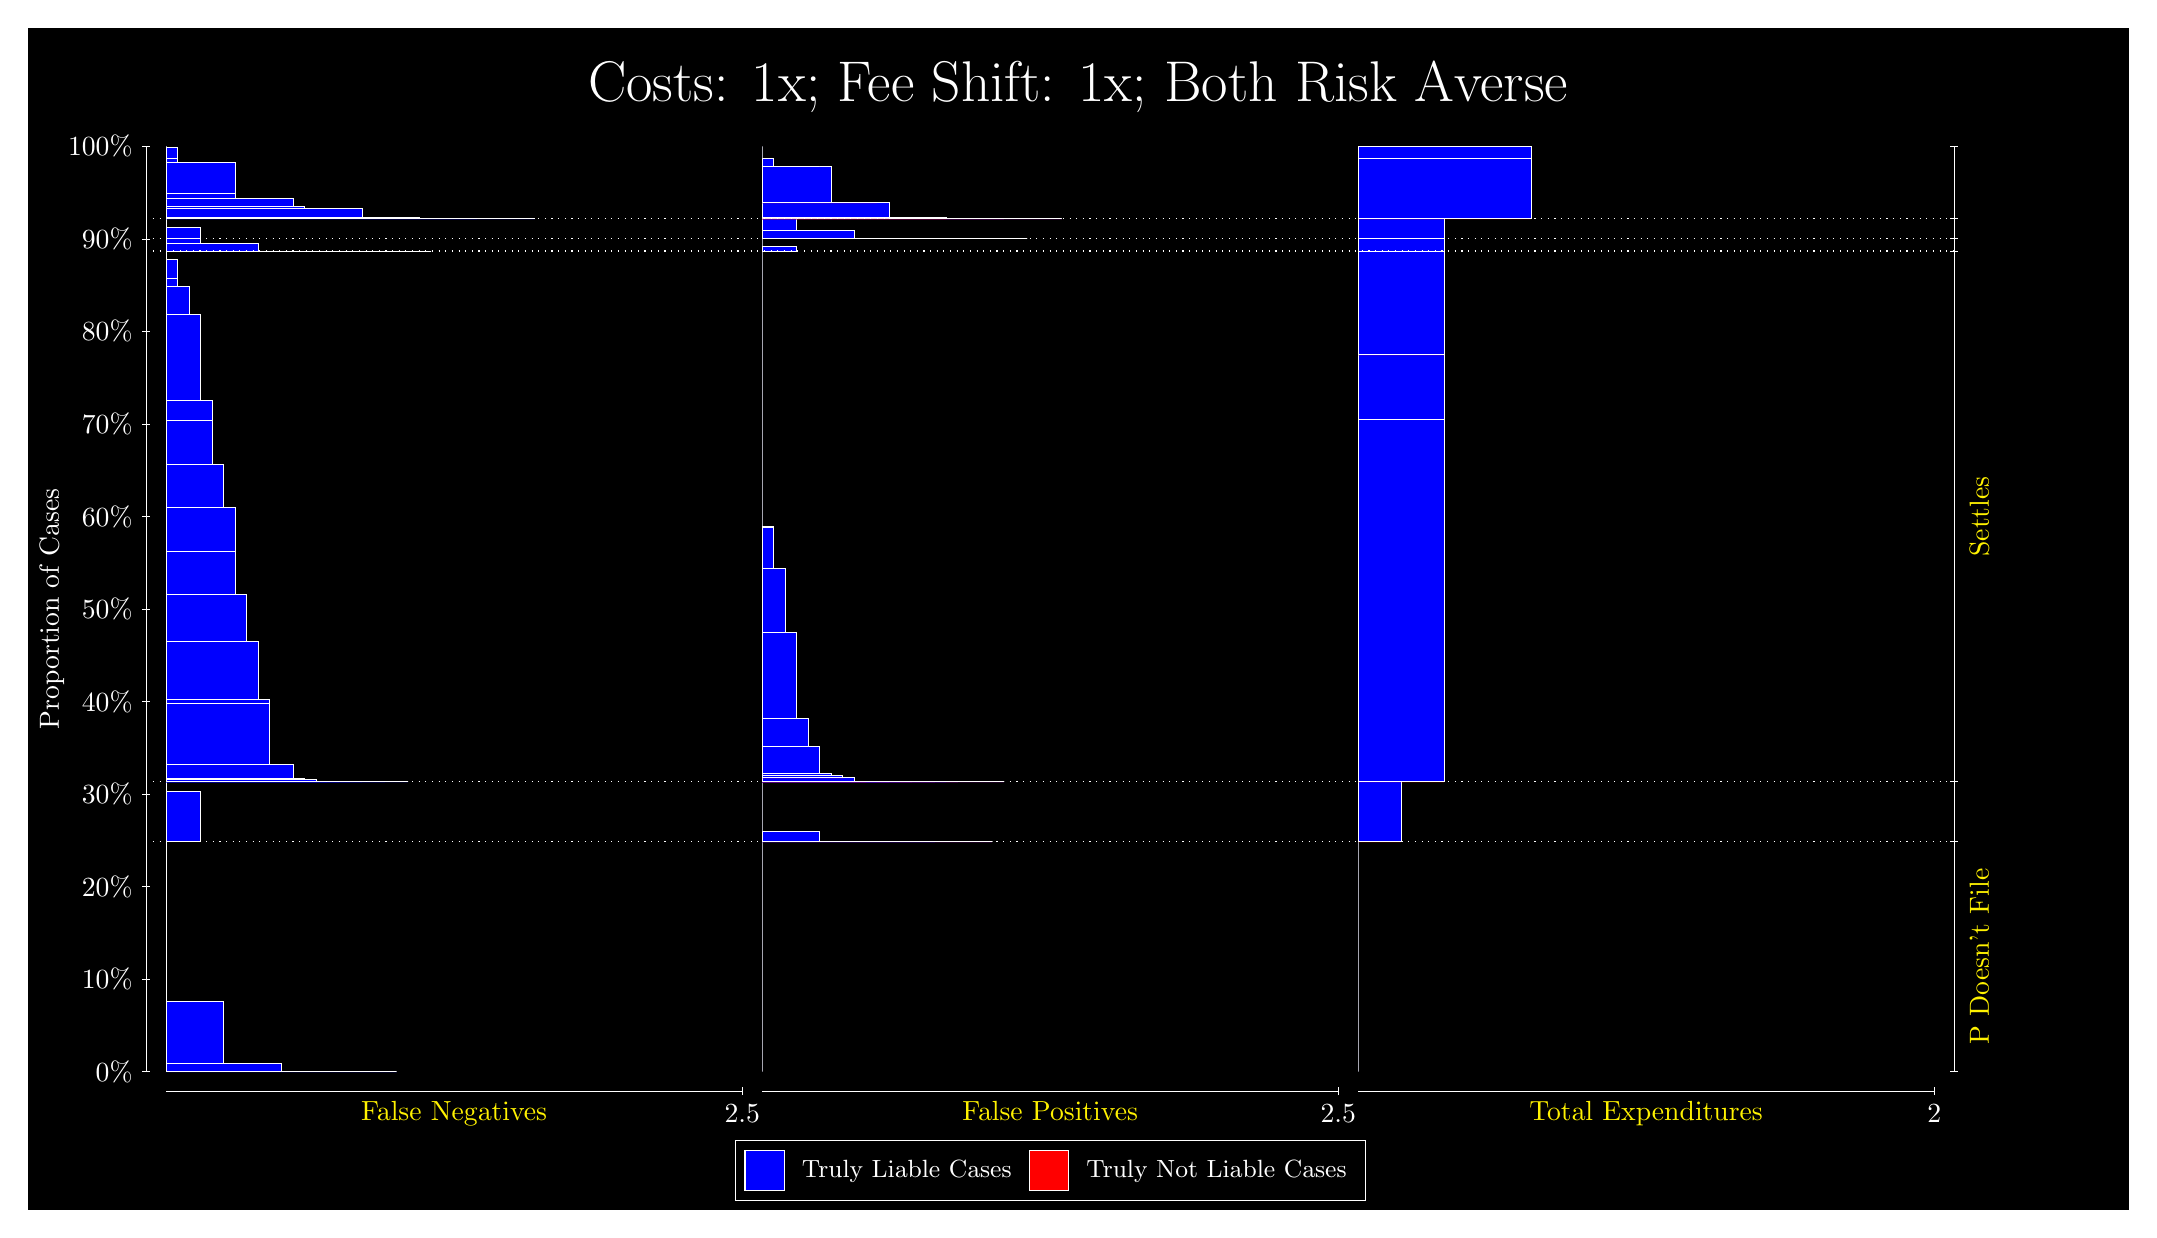
\begin{tikzpicture}
\draw[fill=black] (0,0) rectangle (26.667,15);
\draw[text=white] (0,13.5) rectangle (26.667,15) node[midway] {\huge Costs: 1x; Fee Shift: 1x; Both Risk Averse};
\draw[white, very thin] (1.5,1.75) -- (1.5,13.5);
\node[rotate=90, text=white, anchor=center] at (0.3, 7.625) {Proportion of Cases};
\draw[white, very thin] (1.45,1.75) -- (1.55,1.75);
\node[text=white, anchor=east] at (1.45, 1.75) {0\%};
\draw[white, very thin] (1.45,2.925) -- (1.55,2.925);
\node[text=white, anchor=east] at (1.45, 2.925) {10\%};
\draw[white, very thin] (1.45,4.1) -- (1.55,4.1);
\node[text=white, anchor=east] at (1.45, 4.1) {20\%};
\draw[white, very thin] (1.45,5.275) -- (1.55,5.275);
\node[text=white, anchor=east] at (1.45, 5.275) {30\%};
\draw[white, very thin] (1.45,6.45) -- (1.55,6.45);
\node[text=white, anchor=east] at (1.45, 6.45) {40\%};
\draw[white, very thin] (1.45,7.625) -- (1.55,7.625);
\node[text=white, anchor=east] at (1.45, 7.625) {50\%};
\draw[white, very thin] (1.45,8.8) -- (1.55,8.8);
\node[text=white, anchor=east] at (1.45, 8.8) {60\%};
\draw[white, very thin] (1.45,9.975) -- (1.55,9.975);
\node[text=white, anchor=east] at (1.45, 9.975) {70\%};
\draw[white, very thin] (1.45,11.15) -- (1.55,11.15);
\node[text=white, anchor=east] at (1.45, 11.15) {80\%};
\draw[white, very thin] (1.45,12.325) -- (1.55,12.325);
\node[text=white, anchor=east] at (1.45, 12.325) {90\%};
\draw[white, very thin] (1.45,13.5) -- (1.55,13.5);
\node[text=white, anchor=east] at (1.45, 13.5) {100\%};

\draw[white, very thin] (24.457,1.75) -- (24.457,13.5);
\draw[white, very thin] (24.407,1.75) -- (24.507,1.75);
\node[anchor=west] at (24.407, 1.75) {};
\draw[white, very thin] (24.407,4.6706) -- (24.507,4.6706);
\node[anchor=west] at (24.407, 4.6706) {};
\draw[white, very thin] (24.407,5.4307) -- (24.507,5.4307);
\node[anchor=west] at (24.407, 5.4307) {};
\draw[white, very thin] (24.407,12.17) -- (24.507,12.17);
\node[anchor=west] at (24.407, 12.17) {};
\draw[white, very thin] (24.407,12.331) -- (24.507,12.331);
\node[anchor=west] at (24.407, 12.331) {};
\draw[white, very thin] (24.407,12.582) -- (24.507,12.582);
\node[anchor=west] at (24.407, 12.582) {};
\draw[white, very thin] (24.407,13.5) -- (24.507,13.5);
\node[anchor=west] at (24.407, 13.5) {};

\draw[white, very thin, fill=blue] (1.75,1.75) rectangle (4.6775,1.75);
\draw[white, very thin, fill=blue] (1.75,1.75) rectangle (3.9457,1.7508);
\draw[white, very thin, fill=blue] (1.75,1.7508) rectangle (3.2138,1.8519);
\draw[white, very thin, fill=blue] (1.75,1.8519) rectangle (2.4819,2.6474);
\draw[white, very thin, fill=red] (1.75,2.6474) rectangle (1.75,2.6474);
\draw[white, very thin, fill=blue] (1.75,2.6474) rectangle (1.75,4.6706);
\draw[white, very thin, fill=blue] (1.75,4.6706) rectangle (2.1891,5.3062);
\draw[white, very thin, fill=red] (1.75,5.3062) rectangle (1.75,5.3062);
\draw[white, very thin, fill=blue] (1.75,5.3062) rectangle (1.75,5.4307);
\draw[white, very thin, fill=blue] (1.75,5.4307) rectangle (4.8239,5.4307);
\draw[white, very thin, fill=blue] (1.75,5.4307) rectangle (4.5312,5.4307);
\draw[white, very thin, fill=blue] (1.75,5.4307) rectangle (4.2384,5.4307);
\draw[white, very thin, fill=blue] (1.75,5.4307) rectangle (4.092,5.4307);
\draw[white, very thin, fill=blue] (1.75,5.4307) rectangle (3.9457,5.4307);
\draw[white, very thin, fill=blue] (1.75,5.4307) rectangle (3.7993,5.4307);
\draw[white, very thin, fill=blue] (1.75,5.4307) rectangle (3.6529,5.4586);
\draw[white, very thin, fill=blue] (1.75,5.4586) rectangle (3.5065,5.4789);
\draw[white, very thin, fill=blue] (1.75,5.4789) rectangle (3.3602,5.6488);
\draw[white, very thin, fill=blue] (1.75,5.6488) rectangle (3.2138,5.6497);
\draw[white, very thin, fill=blue] (1.75,5.6497) rectangle (3.0674,6.4291);
\draw[white, very thin, fill=blue] (1.75,6.4291) rectangle (3.0674,6.4818);
\draw[white, very thin, fill=blue] (1.75,6.4818) rectangle (2.921,7.2174);
\draw[white, very thin, fill=blue] (1.75,7.2174) rectangle (2.7746,7.8051);
\draw[white, very thin, fill=blue] (1.75,7.8051) rectangle (2.6283,8.3593);
\draw[white, very thin, fill=blue] (1.75,8.3593) rectangle (2.6283,8.9208);
\draw[white, very thin, fill=blue] (1.75,8.9208) rectangle (2.4819,9.4598);
\draw[white, very thin, fill=blue] (1.75,9.4598) rectangle (2.3355,10.026);
\draw[white, very thin, fill=blue] (1.75,10.026) rectangle (2.3355,10.274);
\draw[white, very thin, fill=blue] (1.75,10.274) rectangle (2.1891,11.368);
\draw[white, very thin, fill=blue] (1.75,11.368) rectangle (2.0428,11.724);
\draw[white, very thin, fill=blue] (1.75,11.724) rectangle (1.8964,11.828);
\draw[white, very thin, fill=blue] (1.75,11.828) rectangle (1.8964,12.062);
\draw[white, very thin, fill=blue] (1.75,12.062) rectangle (1.75,12.063);
\draw[white, very thin, fill=red] (1.75,12.063) rectangle (1.75,12.063);
\draw[white, very thin, fill=blue] (1.75,12.063) rectangle (1.75,12.17);
\draw[white, very thin, fill=blue] (1.75,12.17) rectangle (5.1167,12.17);
\draw[white, very thin, fill=blue] (1.75,12.17) rectangle (4.3848,12.17);
\draw[white, very thin, fill=blue] (1.75,12.17) rectangle (3.6529,12.173);
\draw[white, very thin, fill=blue] (1.75,12.173) rectangle (2.921,12.267);
\draw[white, very thin, fill=blue] (1.75,12.267) rectangle (2.1891,12.331);
\draw[white, very thin, fill=red] (1.75,12.331) rectangle (1.75,12.331);
\draw[white, very thin, fill=blue] (1.75,12.331) rectangle (2.1891,12.474);
\draw[white, very thin, fill=red] (1.75,12.474) rectangle (1.75,12.474);
\draw[white, very thin, fill=blue] (1.75,12.474) rectangle (1.75,12.582);
\draw[white, very thin, fill=blue] (1.75,12.582) rectangle (6.4341,12.582);
\draw[white, very thin, fill=blue] (1.75,12.582) rectangle (5.7022,12.582);
\draw[white, very thin, fill=blue] (1.75,12.582) rectangle (4.9703,12.598);
\draw[white, very thin, fill=blue] (1.75,12.598) rectangle (4.8239,12.598);
\draw[white, very thin, fill=blue] (1.75,12.598) rectangle (4.2384,12.715);
\draw[white, very thin, fill=blue] (1.75,12.715) rectangle (4.092,12.715);
\draw[white, very thin, fill=blue] (1.75,12.715) rectangle (3.5065,12.734);
\draw[white, very thin, fill=blue] (1.75,12.734) rectangle (3.3602,12.837);
\draw[white, very thin, fill=blue] (1.75,12.837) rectangle (2.7746,12.837);
\draw[white, very thin, fill=blue] (1.75,12.837) rectangle (2.6283,12.903);
\draw[white, very thin, fill=blue] (1.75,12.903) rectangle (2.6283,13.295);
\draw[white, very thin, fill=blue] (1.75,13.295) rectangle (2.0428,13.295);
\draw[white, very thin, fill=blue] (1.75,13.295) rectangle (1.8964,13.347);
\draw[white, very thin, fill=blue] (1.75,13.347) rectangle (1.8964,13.486);
\draw[white, very thin, fill=red] (1.75,13.486) rectangle (1.75,13.486);
\draw[white, very thin, fill=blue] (1.75,13.486) rectangle (1.75,13.5);
\draw[white, very thin, fill=red] (9.3189,1.75) rectangle (9.3189,1.75);
\draw[white, very thin, fill=blue] (9.3189,1.75) rectangle (9.3189,4.6706);
\draw[white, very thin, fill=red] (9.3189,4.6706) rectangle (12.246,4.6706);
\draw[white, very thin, fill=blue] (9.3189,4.6706) rectangle (12.246,4.6706);
\draw[white, very thin, fill=blue] (9.3189,4.6706) rectangle (11.515,4.6706);
\draw[white, very thin, fill=blue] (9.3189,4.6706) rectangle (10.783,4.6717);
\draw[white, very thin, fill=blue] (9.3189,4.6717) rectangle (10.051,4.7951);
\draw[white, very thin, fill=blue] (9.3189,4.7951) rectangle (9.3189,5.4307);
\draw[white, very thin, fill=red] (9.3189,5.4307) rectangle (12.393,5.4307);
\draw[white, very thin, fill=blue] (9.3189,5.4307) rectangle (12.393,5.4307);
\draw[white, very thin, fill=red] (9.3189,5.4307) rectangle (11.807,5.4307);
\draw[white, very thin, fill=blue] (9.3189,5.4307) rectangle (11.807,5.4307);
\draw[white, very thin, fill=blue] (9.3189,5.4307) rectangle (11.661,5.4307);
\draw[white, very thin, fill=red] (9.3189,5.4307) rectangle (11.515,5.4307);
\draw[white, very thin, fill=blue] (9.3189,5.4307) rectangle (11.515,5.4307);
\draw[white, very thin, fill=red] (9.3189,5.4307) rectangle (11.222,5.4307);
\draw[white, very thin, fill=blue] (9.3189,5.4307) rectangle (11.222,5.4307);
\draw[white, very thin, fill=blue] (9.3189,5.4307) rectangle (11.075,5.4307);
\draw[white, very thin, fill=blue] (9.3189,5.4307) rectangle (10.929,5.4307);
\draw[white, very thin, fill=red] (9.3189,5.4307) rectangle (10.929,5.4307);
\draw[white, very thin, fill=blue] (9.3189,5.4307) rectangle (10.929,5.4307);
\draw[white, very thin, fill=blue] (9.3189,5.4307) rectangle (10.783,5.4308);
\draw[white, very thin, fill=red] (9.3189,5.4308) rectangle (10.636,5.4308);
\draw[white, very thin, fill=blue] (9.3189,5.4308) rectangle (10.636,5.4413);
\draw[white, very thin, fill=blue] (9.3189,5.4413) rectangle (10.49,5.4812);
\draw[white, very thin, fill=red] (9.3189,5.4812) rectangle (10.344,5.4812);
\draw[white, very thin, fill=blue] (9.3189,5.4812) rectangle (10.344,5.5168);
\draw[white, very thin, fill=blue] (9.3189,5.5168) rectangle (10.197,5.5376);
\draw[white, very thin, fill=blue] (9.3189,5.5376) rectangle (10.197,5.5384);
\draw[white, very thin, fill=red] (9.3189,5.5384) rectangle (10.051,5.5384);
\draw[white, very thin, fill=blue] (9.3189,5.5384) rectangle (10.051,5.8763);
\draw[white, very thin, fill=blue] (9.3189,5.8763) rectangle (9.9044,6.2326);
\draw[white, very thin, fill=blue] (9.3189,6.2326) rectangle (9.758,7.3269);
\draw[white, very thin, fill=blue] (9.3189,7.3269) rectangle (9.6116,8.1406);
\draw[white, very thin, fill=blue] (9.3189,8.1406) rectangle (9.4652,8.6582);
\draw[white, very thin, fill=blue] (9.3189,8.6582) rectangle (9.4652,8.6797);
\draw[white, very thin, fill=blue] (9.3189,8.6797) rectangle (9.3189,12.17);
\draw[white, very thin, fill=red] (9.3189,12.17) rectangle (9.758,12.17);
\draw[white, very thin, fill=blue] (9.3189,12.17) rectangle (9.758,12.234);
\draw[white, very thin, fill=blue] (9.3189,12.234) rectangle (9.3189,12.331);
\draw[white, very thin, fill=red] (9.3189,12.331) rectangle (12.686,12.331);
\draw[white, very thin, fill=blue] (9.3189,12.331) rectangle (12.686,12.331);
\draw[white, very thin, fill=blue] (9.3189,12.331) rectangle (11.954,12.331);
\draw[white, very thin, fill=blue] (9.3189,12.331) rectangle (11.222,12.332);
\draw[white, very thin, fill=blue] (9.3189,12.332) rectangle (10.49,12.439);
\draw[white, very thin, fill=blue] (9.3189,12.439) rectangle (9.758,12.582);
\draw[white, very thin, fill=red] (9.3189,12.582) rectangle (13.125,12.582);
\draw[white, very thin, fill=blue] (9.3189,12.582) rectangle (13.125,12.582);
\draw[white, very thin, fill=red] (9.3189,12.582) rectangle (12.393,12.582);
\draw[white, very thin, fill=blue] (9.3189,12.582) rectangle (12.393,12.582);
\draw[white, very thin, fill=red] (9.3189,12.582) rectangle (11.661,12.582);
\draw[white, very thin, fill=blue] (9.3189,12.582) rectangle (11.661,12.595);
\draw[white, very thin, fill=red] (9.3189,12.595) rectangle (10.929,12.595);
\draw[white, very thin, fill=blue] (9.3189,12.595) rectangle (10.929,12.786);
\draw[white, very thin, fill=red] (9.3189,12.786) rectangle (10.783,12.786);
\draw[white, very thin, fill=blue] (9.3189,12.786) rectangle (10.783,12.786);
\draw[white, very thin, fill=blue] (9.3189,12.786) rectangle (10.197,13.245);
\draw[white, very thin, fill=red] (9.3189,13.245) rectangle (10.051,13.245);
\draw[white, very thin, fill=blue] (9.3189,13.245) rectangle (10.051,13.245);
\draw[white, very thin, fill=blue] (9.3189,13.245) rectangle (9.4652,13.347);
\draw[white, very thin, fill=red] (9.3189,13.347) rectangle (9.3189,13.347);
\draw[white, very thin, fill=blue] (9.3189,13.347) rectangle (9.3189,13.5);
\draw[white, very thin, fill=red] (16.888,1.75) rectangle (16.888,1.75);
\draw[white, very thin, fill=blue] (16.888,1.75) rectangle (16.888,4.6706);
\draw[white, very thin, fill=red] (16.888,4.6706) rectangle (17.437,4.6706);
\draw[white, very thin, fill=blue] (16.888,4.6706) rectangle (17.437,5.4307);
\draw[white, very thin, fill=red] (16.888,5.4307) rectangle (17.986,5.4307);
\draw[white, very thin, fill=blue] (16.888,5.4307) rectangle (17.986,10.039);
\draw[white, very thin, fill=red] (16.888,10.039) rectangle (17.986,10.039);
\draw[white, very thin, fill=blue] (16.888,10.039) rectangle (17.986,10.856);
\draw[white, very thin, fill=red] (16.888,10.856) rectangle (17.986,10.856);
\draw[white, very thin, fill=blue] (16.888,10.856) rectangle (17.986,12.17);
\draw[white, very thin, fill=red] (16.888,12.17) rectangle (17.986,12.17);
\draw[white, very thin, fill=blue] (16.888,12.17) rectangle (17.986,12.331);
\draw[white, very thin, fill=red] (16.888,12.331) rectangle (17.986,12.331);
\draw[white, very thin, fill=blue] (16.888,12.331) rectangle (17.986,12.582);
\draw[white, very thin, fill=red] (16.888,12.582) rectangle (19.083,12.582);
\draw[white, very thin, fill=blue] (16.888,12.582) rectangle (19.083,13.347);
\draw[white, very thin, fill=red] (16.888,13.347) rectangle (19.083,13.347);
\draw[white, very thin, fill=blue] (16.888,13.347) rectangle (19.083,13.5);
\draw[white, dotted] (1.5,4.6706) -- (24.457,4.6706);
\draw[white, dotted] (1.5,5.4307) -- (24.457,5.4307);
\draw[white, dotted] (1.5,12.17) -- (24.457,12.17);
\draw[white, dotted] (1.5,12.331) -- (24.457,12.331);
\draw[white, dotted] (1.5,12.582) -- (24.457,12.582);
\draw[white, very thin] (1.75,1.5) -- (9.0689,1.5);
\node[text=yellow, anchor=north] at (5.4094, 1.5) {False Negatives};
\draw[white, very thin] (9.0689,1.45) -- (9.0689,1.55);
\node[text=white, anchor=north] at (9.0689, 1.45) {2.5};

\draw[white, very thin] (9.3189,1.5) -- (16.638,1.5);
\node[text=yellow, anchor=north] at (12.978, 1.5) {False Positives};
\draw[white, very thin] (16.638,1.45) -- (16.638,1.55);
\node[text=white, anchor=north] at (16.638, 1.45) {2.5};

\draw[white, very thin] (16.888,1.5) -- (24.207,1.5);
\node[text=yellow, anchor=north] at (20.547, 1.5) {Total Expenditures};
\draw[white, very thin] (24.207,1.45) -- (24.207,1.55);
\node[text=white, anchor=north] at (24.207, 1.45) {2};

\node[text=yellow, centered, rotate=90] at (24.777, 3.2103) {P Doesn't File};

\node[text=yellow, centered, rotate=90] at (24.777, 8.8002) {Settles};




\draw (12.978300999999998,1.5) node[draw=none] (baseCoordinate) {};
\begin{scope}[align=center]
        \matrix[scale=0.5, draw=white, below=0.5cm of baseCoordinate, nodes={draw}, column sep=0.1cm]{
            \node[rectangle, draw, minimum width=0.5cm, minimum height=0.5cm, fill=blue] {}; &
            \node[draw=none, font=\small, text=white] (B) {Truly Liable Cases}; &
            \node[rectangle, draw, minimum width=0.5cm, minimum height=0.5cm, fill=red] {}; &
            \node[draw=none, font=\small, text=white] (B) {Truly Not Liable Cases}; \\
            };
\end{scope}

\end{tikzpicture}
\end{document}